\chapter{Short-term residential load forecasting : state of the art}
\label{cha:State of the art short-term residential load forecasting techniques}
As discussed in the introduction, forecasting an individual household is a complex task due to the high uncertainty and volatility of the load signal. To tackle the electrical consumption forecasting, problem neural networks are applied. These models allow for learning very non-linear relations between the inputs and output. Learning is done by updating the model every time such that the observations in the training set are better explained. In this chapter first, an introduction is given about neural networks and the difficulties and solutions are discussed in Section \ref{s:Problems}. Next follows the explanation of the more advanced LSTM and GRU neural networks in respectively Section \ref{s:LSTM} and \ref{s:GRU}, which are specialized in handling time series data. Finally, the introduction to neural networks ends with the explanation of what was found in literature concerning the performance of different parameter settings and different LSTM neural networks in Section \ref{s:Performance results between different models}. The second part of the literature study covers the use of LSTM models for short-term residential electrical load forecasting in Section \ref{s:Short-Term residential electrical load forecasting}.

%Forecasting the electrical load of the individual households presents several challenges. There should be dealt with the missing values, as discussed in section \ref{s:missing_data}. Also, the different time-series are influenced by exogenous factors as weather conditions and calendar information. The dependency on exogenous variables can be a very non-linear relation and can have different effects on different households. Only three indications of the temperature are given on a daily basis. Some additional information is known of certain households, but this data is very incomplete as discussed in Section \ref{s:Identification of driving attributes}. The individual load series have a high volatility and uncertainty compared to a load signal on transmission level which shows more consistent seasonality and straight forward dependency on weather and calendar variables. This makes sense because of the human behavior dependency of the individual household data, while transmission load data are aggregated and uncertainty cancels out.n this thesis, the goal is to investigate individual household. To tackle the high non-linearity that is inherent to residential load forecasting in literature often neural networks are used.
%\textbf{See also paper TA2 --> aggregated vs individual forecasting.}

\section{Introduction to neural networks}\label{s:Introduction to neural networks}
\subsection{MLP}
The simplest configuration of neural networks are multilayer perceptrons and they are made up out of multiple fully connected layers of neurons. Figure \ref{fig:MLP} shows a MLP with one hidden layer.

\begin{figure}[h!]
	\centering
	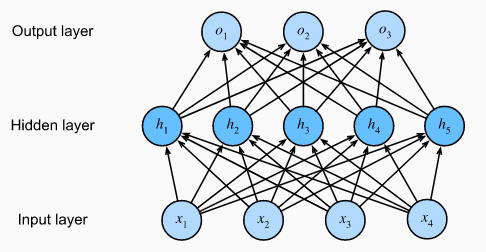
\includegraphics[width=0.8\textwidth]{MLP.png}
	\caption{Figure of a MLP (source \cite{Czum2020}).}
	\label{fig:MLP}
\end{figure}

All layers are connected to the next layer by the means of an affine function together with a non-linear activation function represented by sigma as shown by equation \ref{eq:NN} with $ \textbf{L}^{(N)} $ the vector with outputs of the Nthe layer, $ \textbf{W}^(N) $ the Nth weight matrix and $ \textbf{b}^{(N)} $ the Nth bias

%It can be noted that the MLP network is invariant.

\begin{equation}\label{eq:NN}
	\textbf{L}^{N+1} = \sigma(\textbf{W}^{(N)}\textbf{L}^{N}+\textbf{b}^{(N)}).
\end{equation}

A  standard multilayer feedforward neural network with locally bounded piecewise continuous activation function can approximate any continuous function to any degree of accuracy if and only if the network's activation function is not a polynomial, as stated by \textbf{Leshno et al} in \textbf{1993}. This theorem proves that a ``universal approximator'' exists for continuous functions, but it lacks the recipe to construct it. In \cite{Nielsen2015} it is shown that a feedforward network with a single layer is enough to approximate any function by a specified accuracy if the hidden layer has the possibility to add an unlimited amount of hidden neurons in its layer. It is discussed that when a function is discontinuous, which means that it makes sudden, sharps jumps, it is not possible to approximate the function by any prescribed accuracy. However, in practise a continuous approximation is often good enough.\\

Neural networks are suitable of learning very non-linear mappings between inputs and outputs. The difference between ``Deep neural networks'' and ``Shallow neural networks'' is the amount of layers of neurons that are used inside the network. The layers of neurons, that are not inputs or outputs are called ``hidden neurons''. Because a ``Deep neural network'' has a hierarchical layout of the different hidden layers, it not only learning features from the non-linear combinations of inputs, but uses other layers to learn features of combinations of features learned in lower hidden layers. This is possible because higher hidden layers get the outputs of lower hidden layers as input. However, because of the higher expressiveness, a ``Deep neural network'' with respect to a ``Shallow neural network'', suffers more of overfitting as is discussed in section \ref{s:Problems}.


\subsection{RNN}\label{s:RNN}
A recurrent neural network is a specialized neural network to deal with sequential information. The output of recurrent neural networks depend on the prior elements within the sequence. In order to take past information from previous inputs into account, a hidden variable $ \bm{H}^t $ is used. By making use of this variable which makes a summary of the previous seen information, a large increase in the number of model parameters is avoided. Cited from \cite{bibid}: ``Hidden states are technically speaking inputs to whatever we do at a given step, and they can only be computed by looking at data of previous time steps''. Equation \ref{eq:RNN} shows how the previous hidden state and the current information are merged in the next hidden state with $ \textbf{X}^t\in \mathbb{R}^{d} $, $ \textbf{H}^t\in \mathbb{R}^{h} $, $ \textbf{W}_1\in \mathbb{R}^{h\times d} $, $\textbf{W}_2\in \mathbb{R}^{h\times h} $ and $ \textbf{b}\in \mathbb{R}^{h} $ 

\begin{equation}\label{eq:RNN}
	\textbf{H}^{t+1} = \tanh(\textbf{W}_1\textbf{X}^{t}+\textbf{W}_2\textbf{H}^{t}+\textbf{b}).
\end{equation}

The equation $\textbf{X}^t$ corresponds to one input at time step $ t $ with dimensionality $ d $. 
Also a deep RNN is possible, where multiple layers and hidden states are used per time step. \\

\begin{figure}[h]
	\centering
	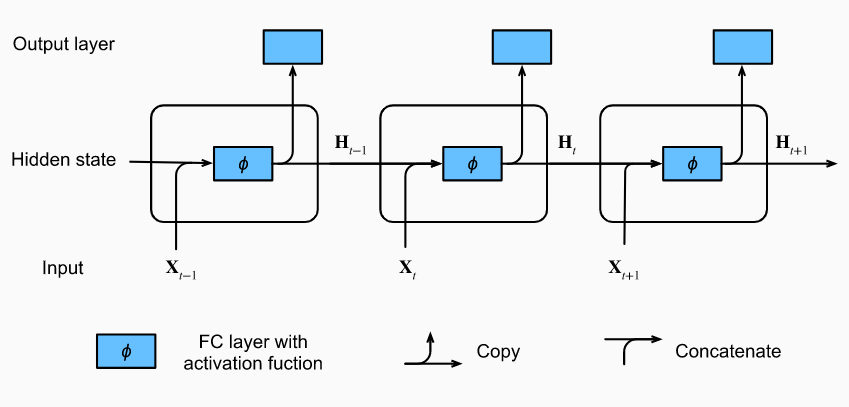
\includegraphics[width=1.0\textwidth]{RNN.png}
	\caption{Vanilla RNN,(source: \cite{Czum2020}).}
	\label{fig:RNN}
\end{figure}

As was discussed in the beginning of this section a standard neural network can act as a ``universal approximator'' when given enough hidden states. A similar result exist for a recurrent neural network which states that it is capable to approximate a sequence-to-sequence mapping to an arbitrary accuracy as discussed in \cite{Hammer2000}. However, as discussed in \cite{Teuwen2019} even if expressiveness of the simple model is very powerful in theory, this doesn't indicate that such a representation can be learn in a reasonably amount of time from a dataset. As will be discussed in Section \ref{s:Problems}, the main drawback of the vanilla recurrent neural network is that it forgets fast important information in function of the amount of time steps. When using ``backpropagation through time'' for updating the weights, the gradients that corresponds to inputs seen a lot of time steps ago will become very small due to the multiplication of small gradients over the time steps. Therefore, their contribution of updating the weights of the recurrent neural network will be very small and thus this information will be ``forgotten''.


\subsection{Difficulties \& Solutions of neural networks}\label{s:Problems}
Neural networks have a high expressiveness but this comes at the cost of overfitting and a vanishing gradient.
when the neural network is learning from training data, every epoch the error between the input and output of the training examples is reduced. In the beginning the validation error reduces simultaneously with the training error. The validation error is the error that the model makes on data that is not seen during training. On a certain point during the training the validation error increases while the training error still decreases. This means that the model is no longer learning intelligent general rules and patterns in the data, but it starts remembering the training data and therefore the model will not perform well in general. This is often the case in a model with an high expressiveness because the model is less pushed to make generalizations and has the ability to just remember the training data. Solutions to overfitting can be regularization which includes the weight sizes as a cost in the objective function. Typical choices for resembling the size of the weights are the $ L_1 $ and the $ L_2 $ norms. Other methods that can be used are: early stopping, dropout and pruning.

It should be noted that the gradient can increase very much over the different time steps, which in literature is called gradient explosion. The solution strategy for this is applying gradient clipping by norm or by value. Gradient clipping by norm means that when the 2-norm of the gradient $ \bm{\xi} $ exceeds a threshold value $ \theta $, the 2-norm of the gradient is scaled to equal the threshold value. The mathematical formulation is given by equation \ref{eq:clipping}:

\begin{equation}\label{eq:clipping}
	\bm{\xi}= min(1,\frac{\theta}{\| \bm{\xi} \|})\times\bm{\xi}.
\end{equation}

An alternative method to avoid gradient explosion is using gradient value clipping. The second problem is the vanishing gradient which in a RNN setting corresponds to having a short term memory which means that initial inputs that were presented to the neural network are being forgotten. This can be mitigatedd using a LSTM or GRU. Both techniques have in common that they can learn which data in the sequence is important and should be retained and which information can be thrown away. It is important to state that LSTM and GRU are not solving the vanishing gradient problem as explained in \cite{Teuwen2019}. The gradient is still exponentially decreasing, but the effect is less pronounced as can be seen for LSTM in Figure \ref{fig:grad_exp}. When the forget gate, that sits inside a LSTM cell outputs a value that is close to one, the exponential decay will have also a base close to one. $ \tau $ gives the number of epochs. As discussed in \cite{Teuwen2019}, the amount of memory and calculation effort needed to do a gradient update increases linearly with the amount of time steps. Memory and calculation load can be mitigated by making use of truncated backpropagation through time.\\  
% The second problem is the vanishing gradient which originates because while using the backpropagation algorithm to calculate the gradient which is used in different update methods of the weights, the gradient is calculated at the end of the neuaral network and propagated back using every time the previous calculated gradient values which exponentially decreases in function of the time steps. Therefore, at the first layers of the network, the gradient has become so small that the weights are almost not updated anymore.

%The complexity of the recurrent models grows linearly with the amount of time steps that are processed in the sequence.

\begin{figure}[h!]
	\centering
	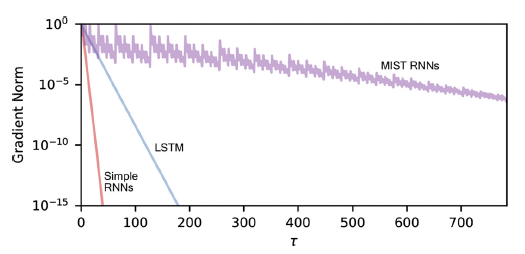
\includegraphics[width=0.8\textwidth]{grad_exp.png}
	\caption{Exponential decrease of the gradient size of a simple RNN (red) or a LSTM (blue) (source: \cite{Teuwen2019}).}
	\label{fig:grad_exp}
\end{figure}


\subsection{LSTM}\label{s:LSTM}

\begin{figure}[ht]
	\centering
	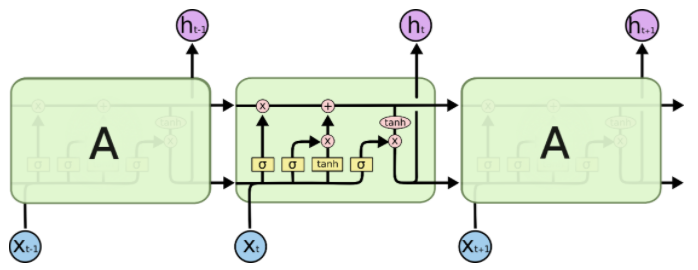
\includegraphics[width=1.0\textwidth]{LSTM_cell.png}
	\caption{A LSTM cell that is repeated over time (source: \cite{Olah}).}
	\label{fig:LSTM_cell}
\end{figure}

As discussed in Section \ref{s:Problems}, the LSTM is an updated version of the conventional RNN first proposed by \textbf{Hochreiter \& Schmidhuber} in $ 1997 $ to deal with the short term memory a RNN suffers from. A LSTM can longer take important aspects of the presented time series into account which can be used during prediction. To do this a LSTM makes use of three gates: forget gate $ \textbf{f}_t $, input gate $ \textbf{i}_t $ and an output gate $ \textbf{o}_t $. When comparing the three gates with Eq. \ref{eq:RNN}, it is clear that every gate is by itself a recurrent neural network, with the only difference that a sigmoid function is used instead of a hyperbolic tangent. The core concept of the LSTM is that it makes use of a memory cell that is passed on through the different time steps. The memory cell contains important information that is seen before in the data and should be taken into account at the current new output. The three gates can delete, write and read information from this memory cell. It can also be noted that Eq. \ref{LSTM_rnn} is exactly equal to the conventional RNN described by Eq. \ref{eq:RNN}. Eq. \ref{LSTM_rnn} processes the hidden states $ \bm{H}_t $ and the new input $ \bm{X}_t $ to propose an update $ \tilde{\textbf{c}}_t $ to the previous memory cell. The input gate Eq. \ref{LSTM_input} decides what will be preserved of the proposal and actually updated. The forget gate Eq. \ref{LSTM_forget} decides what will be preserved from the original memory cell $ \textbf{c}_t $. When both the old memory cell and the proposal are pruned, they are combined to one new memory cell. This new memory cell is together with the output gate Eq. \ref{LSTM_output} used to output new hidden states. \\

In order to train a LSTM neural network there are considerably more parameters that have to be learned than a conventional RNN. An LSTM has four different weight matrices for both the hidden states and the inputs. Because by this increase of weights also the expressiveness of the model has increased with respect to the vanilla recurrent neural network of Section \ref{s:RNN}. Therefore, overfitting of the data should be extra monitored. The LSTM equations are given as follows as they were found in \cite{Teuwen2019}:
\begin{equation}\label{LSTM_forget}
	\textbf{f}_{t} = \sigma(\textbf{W}_{fH}\textbf{H}_{t-1}+\textbf{W}_{fX}\textbf{X}_{t-1}+\textbf{b}_{f}),
\end{equation}
\begin{equation}\label{LSTM_input}
	\textbf{i}_{t} = \sigma(\textbf{W}_{iH}\textbf{H}_{t-1}+\textbf{W}_{iX}\textbf{X}_{t-1}+\textbf{b}_{i}),
\end{equation}
\begin{equation}\label{LSTM_output}
	\textbf{o}_{t} = \sigma(\textbf{W}_{oH}\textbf{H}_{t-1}+\textbf{W}_{oX}\textbf{X}_{t-1}+\textbf{b}_{o}),
\end{equation}
\begin{equation}\label{LSTM_rnn}
	\tilde{\textbf{c}}_{t} = \tanh(\textbf{W}_{cH}\textbf{H}_{t-1}+\textbf{W}_{cX}\textbf{X}_{t-1}+\textbf{b}_{c}),
\end{equation}
\begin{equation}\label{LSTM_memory}
	\textbf{c}_t = \textbf{f}_t\times\textbf{c}_{t-1}+\textbf{i}_t\times\tilde{\textbf{c}}_t,
\end{equation}
\begin{equation}\label{LSTM_next}
	\textbf{H}_t = \textbf{o}_t\times\tanh(\textbf{c}_t).
\end{equation}


%Further, it can also be noted when looking to the LSTM equations that when the parameter that determines the amount of hidden states this will have a higher effect on the calculation load of a LSTM than the vanilla RNN. This is similar when more inputs are added.

\subsection{GRU}\label{s:GRU}

\begin{figure}[ht]
	\centering
	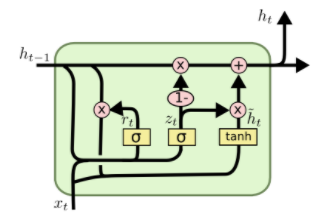
\includegraphics[width=0.6\textwidth]{GRU_cell.png}
	\caption{A GRU cell that is repeated over time (source: \cite{Olah}).}
	\label{fig:GRU_cell}
\end{figure}
A gated recurrent unit neural network is a newer, simplified version of the LSTM that deals with the short term memory problem of a vanilla recurrent neural network. It was introduced by \textbf{Cho et al.} in $ 2014 $. The LSTM is changed by merging the forget and input gate into an update gate. Also, the memory cell and hidden states are combined. The difference in performance between variations of the LSTM neural network is discussed in Section \ref{s:Performance results between different models}. The following GRU equations are as found in \cite{Teuwen2019}:

\begin{equation}
	\textbf{z}_{t} = \sigma(\textbf{W}_{zH}\textbf{H}_{t-1}+\textbf{W}_{zX}\textbf{X}_{t-1}+\textbf{b}_{z}),
\end{equation}
\begin{equation}
	\textbf{r}_{t} = \sigma(\textbf{W}_{rH}\textbf{H}_{t-1}+\textbf{W}_{rX}\textbf{X}_{t-1}+\textbf{b}_{r}),
\end{equation}
\begin{equation}
	\tilde{\textbf{H}}_{t}=\tanh(\textbf{W}_{HH}(\textbf{r}_t\times\textbf{H}_{t-1})+\textbf{W}_{HX}\textbf{X}_t+\textbf{b}_H),
\end{equation}
\begin{equation}
	\textbf{H}_t=\textbf{z}_t\times\textbf{H}_{t-1}+(1-\textbf{z}_t)\times\tilde{\textbf{H}}_t.
\end{equation}

\subsection{Performance of different parameter settings and variations of LSTM neural network models from literature}\label{s:Performance results between different models}
Paper \cite{Chung2014} conducts an empirical evaluation of the GRU and compares it with the older LSTM. It was found that it outperformed the vanilla RNN and attained similar performance as the LSTM on the task of polyphonic music modelling and speech signal modelling. 
According to \cite{Olah}, the next step in sequence modelling is the use of attention models or grid LSTM's.\\

There exists a lot of variations of the LSTM neural networks. Paper \cite{Greff2017} discusses a large-scale analysis of eight LSTM variants on the tasks of: speech recognition, handwritting recognition and polyphonic music modelling. The hyperparameters of the models were optimized using a random search method. The influence of each of the hyperparameters was assessed using the fANOVA toolbox. This toolbox is in more detail explained in \cite{Hutter2014}. It was found that none of the assessed variants could significantly outperform the conventional LSTM architecture. However, it was stated that the LSTM variants in some occasions were able to simplify the calculation load and number of parameters, without the lost of performance. Next, it was found that the forget and output gate were the most crucial gates of the LSTM network. When one of the two was removed, a significant lost of performance occurred. There was also an hyperparameter search conducted with following hyperparameters:

\begin{itemize}
	\item Amount of LSTM hidden states
	\item Learning rate
	\item Momentum term
	\item Standard deviation of Gaussian input noise
\end{itemize}

It was concluded that it can be assumed that there is no interaction between the different parameters. The largest interaction could be found between the learning rate and the amount of LSTM hidden states, which was still small. Therefore, parameters can be varied individually which can drastically reduce the amount of runs that had to be performed to see the effect on the model. Next, it was concluded that the learning rate was the most important parameter and could be tuned by setting it initially high e.g. to 1, and then let it decreases until the error on a validation set starts increasing. The use of a momentum term, which takes previous values of the weights into account when updating, was found to be unimportant in their setting of online gradient descent. The use of gaussian input noise to avoid overfitting was found to be not helpful. 

\section{Short-Term residential electrical load forecasting}\label{s:Short-Term residential electrical load forecasting}

%Classical ways to deal with uncertainty.\\
%Residential electrical load series have a high amount of volatility and uncertainty due to the contingency of the electrical consumption. Classical ways to deal with this are discussed in \cite{Shi2018} and listed as follows:

%\begin{enumerate}
% \textbf{But the uncertainty on the whole is reduced --> on single household stays the same!!}
%	\item Aggregating the residential loads to cancel out the uncertainties. The aggregated signal will show more regular patterns which means that is easier to predict.The downside is that the aggregated forecast will do a poor job of serving as forecast for a household
%	\item A spectral analysis e.g. wavelet analysis, Fourier transforms and empirical mode decomposition aim at seperating a load serie into a regular pattern, an uncertain signal and noise. Because the amount of regularity is low in a residential load serie, this method is infeasible.
%\end{enumerate}

In paper \cite{Shi2018} a novel pooling-based deep recurrent neural network is proposed which collects load profiles of neighbouring houses into a pool of training inputs. Pooling of neighbouring households historical load to serve as input of a deep LSTM neural network, is proposed to increase the data volume and diversity of the training set. The goal of using a pooled training set is to avoid overfitting present when using a deep LSTM neural network. Regarding notation, LSTM is used here instead of RNN with LSTM units as done in the paper. The idea is as quoted by \cite{Shi2018}, to use the interconnected spacial information to compensate insufficient temporal information. The pool of data allows to learn the correlations between neighbouring households and the shared uncertainties coming from external factors. Pools consisting out of $ 10 $ households are used. From the pool of inputs every epoch a randomly chosen batch is fed to the LSTM network. Training is stopped when the MSE on the training set is converged. When the training ends, performance is tested for each household in the pool.\\

%An overview of the different steps that were done during the proposed method are: data cleaning and preprocessing $\rightarrow$ data pooling $\rightarrow$ data sampling $\rightarrow$ data training $\rightarrow$ benchmarking.\\

Performance of the proposed method was evaluated based on a test set of $ 30 $ days and is twofold : 
\begin{enumerate}
	\item Performance of the proposed method with respect to ARIMA, vanilla LSTM, SVR and DLSTM (without pooling)
	\item The effect of the neural network depth and pooling
\end{enumerate}

For the first part of the method evaluation it was concluded that the proposed DLSTM with pooling, outperforms all other methods based on the metrics RMSE, NRMSE and MAE.

%\begin{equation}\label{eq:RMSE}
%	RMSE = \sqrt{\frac{\sum_{t=1}^{N}(\hat{y}_t-y_t)^2}{N}},
%\end{equation}
%\begin{equation}\label{eq:NRMSE}
%	NRMSE = \frac{RMSE}{y_{max}-y_{min}},
%\end{equation}
%\begin{equation}\label{eq:MAE}
%	MAE = \frac{\sum_{t=1}^{N}\abs{\hat{y}_t-y_t}}{N}.
%\end{equation}

The amount of which the PDLSTM outperformed the other methods can be seen in Table \ref{tab:pooling_result}. The effect of the depth of the DLSTM and the pooling method is depicted in Figure \ref{fig:Shi2018_result}. It can be seen that without the pooling method the DLSTM only benefits from extra LSTM layers till three. This is because from that point, overfitting will reduce the generalization capacity of the DLSTM. With the pooling technique, extra layers stays beneficial. It can thus be concluded that introducing extra hidden layers is a good choice to model the non-linear relations, but this can only be done efficiently when overfitting is mitigated by the use of a pooling strategy.The LSTM with pooling used for benchmarking consisted out of five layers and thirty hidden units in each layer.\\

\begin{figure}[h!]
	\centering
	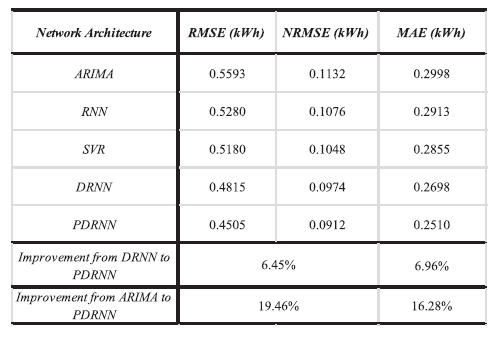
\includegraphics[width=1\textwidth]{pooling_result.png}
	\caption{Comparing different methods in \cite{Shi2018}.}
	\label{tab:pooling_result}
\end{figure}

\begin{figure}[h!]
	\centering
	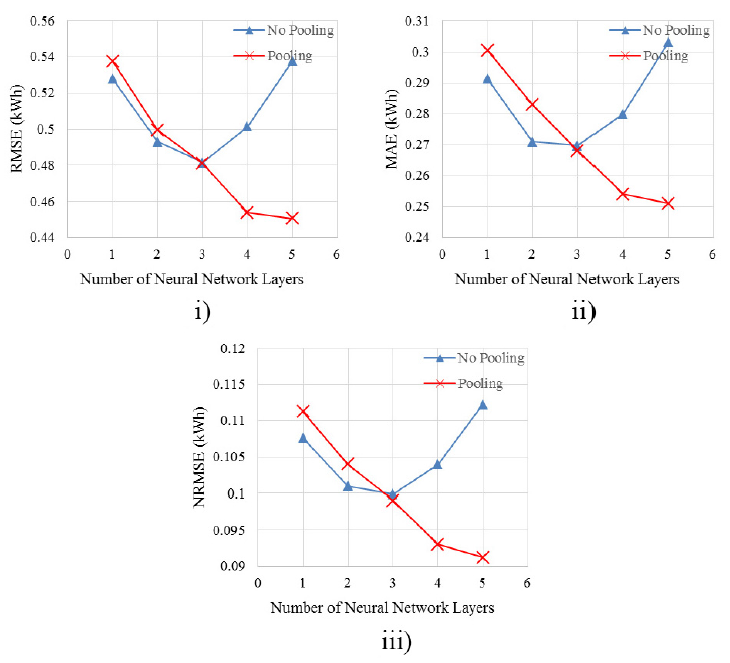
\includegraphics[width=1\textwidth]{Shi2018_result.png}
	\caption{Influence of the number of layers and the pooling method in \cite{Shi2018}.}
	\label{fig:Shi2018_result}
\end{figure}

%GRU (Gated Reset Update) or LSTM (Long Short Term Memory) can be implemented. They are both enhancements of the vanilla RNN which suffers from a vanishing gradient which causes it to to behave without a long term memory. In practise to know which one works often both are tried \cite{Teuwen2019}. Stochastic gradient descent means that the approximated gradient is calculated from a random subset of the available data instead from the entire dataset. \\

%\textbf{Short-term Residential load forecasting based on LSTM RNN paper}\\

In \cite{Kong2019} it is chosen for a deep LSTM approach to forecast the electricity load of a single household. A deep LSTM has multiple LSTM layers. It is first discussed that the aggregated electrical load serie shows more regularity than the load signal of an individual household.  This is substantiated by making use of a density based clustering technique, where it is shown that the different daily consumptions profiles of the aggregated signal could be described by one cluster and no outliers. An outlier means that a daily consumption profile could not be assigned to a cluster. On the other hand for individual household load series, the amount of outliers can range to over $ 80 $. The amount of outliers a load signal has, is a measure of the amount of regularity of the signal.\\
Because the household load signals are characterized by the residents daily routines, this is tried to be learned directly by the deep LSTM.
Inputs that are given to the LSTM are $ k $ past half hour load values, the time of when the measurements were taken, the day of the week and if the day is a holiday or not. In table \ref{tab:LSTM_lit_result} the results are shown of the LSTM method in comparison with other forecasting techniques. It can be seen that the proposed technique outperforms the rest based on the performance when making $ 29,808 $ predictions. Forecasting was performed on $ 69 $ different electrical load series coming from households in Australia. It was concluded that learning methods that had good performance on aggregated time series e.g. IS-HF and KNN (k-nearest neighbour), perform much worse when predicting individual households. \\
By making use of linear regression in function of the amount of outliers, to obtain a measure for consistency, it is shown that LSTM and BPNN (Back-Propagation neural network) perform similar for consistent load signals. The LSTM only starts to differentiate in performance when inconsistency grows and the BPNN is then outperformed. Things that can be improved in \cite{Kong2019} are practical useful forecasts of a timespan of $ 24 $ hours instead of only half an hour and not making use of a rule of thumb during hyperparameter tuning but a hyperparameter search.\\

\begin{figure}[h!]
	\centering
	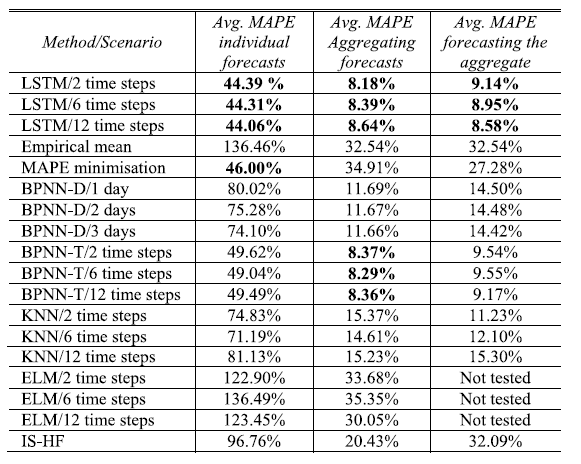
\includegraphics[width=1\textwidth]{prev_appr.png}
	\caption{Different approaches tried in \cite{Kong2019} and their performance in making $ 29,808 $ predictions.}
	\label{tab:LSTM_lit_result}
\end{figure}

\textbf{CNN-LSTM paper}\\
In \cite{Kim2019} a novel technique is proposed which makes use of a convolutional neural network from which the outputs are given to a LSTM recurrent network after which a fully connected neural network  is used to produce the outputs. The purpose of the CNN is to extract the features that are the main drivers of energy consumption and to remove the noise that comes initially together with the raw inputs. The CNN is made up out of convolution layers and pooling layers and makes use of the ``ReLU'' activation function. The main purpose of a convolution layer is to extract features while the pooling layer reduces the number of parameters by making use of the ``max pooling principle''. Using the ``max pooling principle'' means taking the max value of each neuron cluster of the previous layer. As discussed in paper \cite{Kong2019} LSTM is suitable to alleviate the problem of a vanishing or exploding gradient which characterized a simple RNN. LSTM is able to preserve long-term memory by making use of memory states that is used in the calculation of hidden states. It is therefore suitable to remembering the irregular trend of the electrical load time-serie. Finally, a fully connected time-serie predicts the load forecast.\\
Paper \cite{Kim2019} further showed superiority with respect to only making use of the LSTM layers as can be seen in Table \ref{tab:CNN-LSTM_results}. The  Inputs that were used to forecast the household load which is located in France are: three submeters with historical loads, global intensity, voltage, global reactive power, global active power, time, data and month. 
At last, also an analysis is performed to investigate the influence of the different inputs by calculating the average class activation score over the inputs. The results are shown in Figure \ref{fig:LSTM-CNN_results}. It can be seen that especially ``Sub metering $ 3 $'' has a big influence on the final forecasts. This sub meter corresponds to the the electric water heater and air conditioner of the house. As was shown in Section \ref{tab:attributes} the dataset used in this thesis gives only information about the presence of a hot water heater.  Discussed limitations in the paper are the definition of the hyper parameters that were set by trail and error instead of using an automated method e.g. a genetic algorithm. A further limitation is the lack of household characteristics e.g. the amount of residents living in the house. It has previously been shown by \textbf{C. Beckel et al.} that household occupancy is one of the primarily drivers of electrical consumption in a household.\\

\begin{figure}[h!]
	\centering
	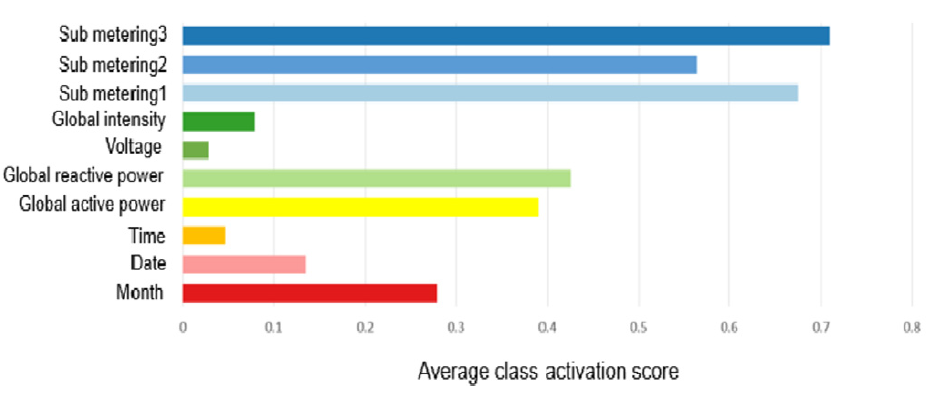
\includegraphics[width=1\textwidth]{CNN-LSTM_results_F.png}
	\caption{The importance of the different inputs as based on the average class activation score. (source \cite{Kim2019})}
	\label{tab:LSTM_lit_results}
\end{figure}

\begin{figure}[h!]
	\centering
	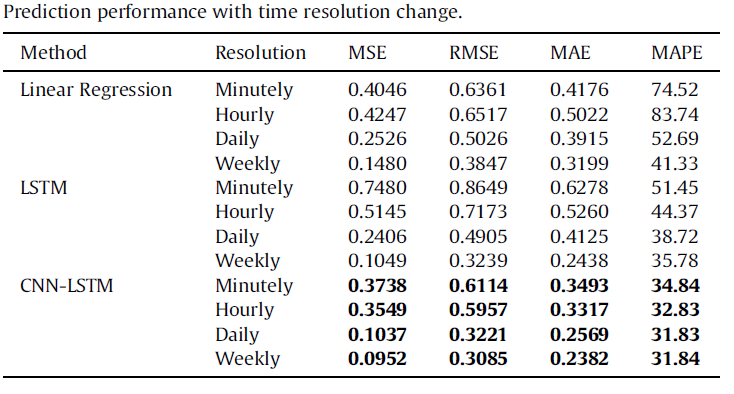
\includegraphics[width=1\textwidth]{CNN-LSTM_results_T.png}
	\caption{Comparison between LSTM and CNN-LSTM. (source: \cite{Kim2019})}
	\label{tab:LSTM_lit_results}
\end{figure}

\textbf{CNN-GRU paper}\\
\cite{Sajjad2020}

\textbf{See oneNote for the summary of the paper and say that it is showed that CNN-GRU performs even better than CNN-LSTM}


\section{Conclusion}
The final section of the chapter gives an overview of the important results
of this chapter. This implies that the introductory chapter and the
concluding chapter don't need a conclusion.



%%% Local Variables: 
%%% mode: latex
%%% TeX-master: "thesis"
%%% End: 
